\section{Related Work}

\paragraph{Intra-image self-supervised training.}
A first family of self-supervised methods focuses on pretext tasks built from the image, i.e., extracting a signal from the image to be predicted from the rest of the image. 
This idea has become prevalent with the work of \cite{doersch2015unsupervised}, where they train by predicting the context of a given patch.
Many other pretext tasks were introduced based on, for example, re-colorizing images~\citep{zhang2016colorful}, predicting transformations~\citep{gidaris2018unsupervised}, inpainting~\citep{pathakCVPR16context} or patch re-ordering~\citep{noroozi2016jigsaw, misra2020self}.
Recently, the emergence of patch-based architectures, like ViTs, has led to a revisit of inpainting for pre-training~\citep{he2021masked, bao2021beit, el2021large}, potentially in feature space~\citep{assran2023self, baevski2022data2vec}.
Of particular interest, \cite{he2021masked} show that a masked auto-encoder~(MAE) learns features that provide substantial improvements when finetuned on downstream tasks.
This property of MAEs has been further validated on video~\citep{tong2022videomae}, audio~\citep{xu2022masked}, and across other modalities~\citep{girdhar2022omnimae}.
However, their features require supervised finetuning, while our features perform well out of the box.

\begin{figure}[t]
  \centering
  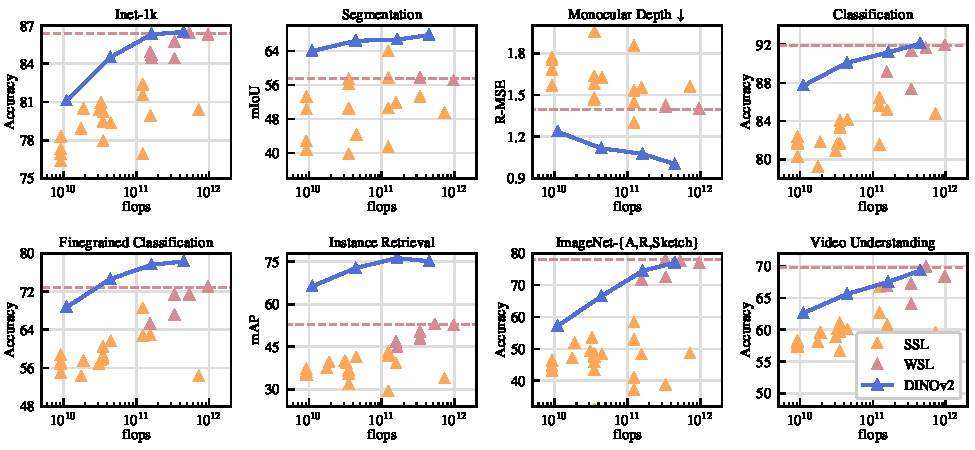
\includegraphics{pullfigure_5.pdf}
  \caption{
    \textbf{Evolution of performance when scaling in parameters.}  
    We show performance on eight types of vision tasks, as presented in Sec.~\ref{sec:results}, and average metrics with each type.
    Features are extracted from our self-supervised encoders, \OURS~(dark blue), and we compare them with self-supervised methods (pale orange), as well as weakly-supervised methods (dark pink). 
    We report the best-performing weakly-supervised model's performance as a dashed horizontal line.
    Our family of models drastically improves over the previous state of the art in self-supervised learning and reaches performance comparable with weakly-supervised features.
    See Sec.~\ref{sec:results} for a detailed analysis.
    \label{tab:pullfig}
  }
\end{figure}

\paragraph{Discriminative self-supervised learning.}
The second line of work, closer to ours, is using discriminative signals between images or groups of images to learn features.
This family of methods has roots in early deep learning work~\citep{hadsell2006dimensionality} but became popular with the emergence of instance classification methods~\citep{dosovitskiy2016discriminative, bojanowski2017unsupervised, wu2018unsupervised}.
Several improvements were made based either on instance-level objectives~\citep{henaff2019data,he2020momentum, chen2020exploring, chen2020simple,grill2020bootstrap, caron2021emerging} or clustering~\citep{caron2018deep,asano2019self, caron2020unsupervised}. 
These methods provide performant frozen features on standard benchmarks like ImageNet~\citep{russakovsky2015imagenet}, but they are hard to scale to larger model sizes~\citep{chen2021empirical}.
In this work, we revisit the training of these approaches in the context of large pretraining datasets and models.
In particular, we build on top of~\cite{zhou2021ibot} that we find particularly suited for scaling.

\paragraph{Scaling self-supervised pretraining.}
A growing body of work has focused on the scaling abilities of self-supervised learning in terms of data and model size~\citep{caron2019unsupervised, goyal2019scaling, tian2021divide, goyal2022vision}.
Most of these works use large quantities of uncurated data to train models without supervision.
They show evidence that discriminative methods scale with data, but because of the poor quality of the pretraining data, most of the results are obtained by finetuning the features.
Of particular interest, \cite{goyal2021self} have also shown that these methods benefit from scaling in model size given enough pretrained data.
This line of work questions the ability of self-supervised methods to work on any data while we focus on producing the best pretrained encoders.

\paragraph{Automatic data curation.}
Our dataset construction borrows from the image retrieval community~\citep{weinzaepfel2021learning,radenovic2018fine,berman2019multigrain,douze2009evaluation,tolias2015particular,revaud2019learning}.
In particular, the use of retrieval to augment the training set has been studied in the context of semi-supervised learning~\citep{yalniz2019billion}.
Similarly, others have used hashtags or other metadata~\citep{mahajan2018exploring,radford2021learning} or pretrained vision encoders~\citep{schuhmann2021laion, schuhmann2022laion} to filter uncurated datasets.
Unlike these works, we use no pretrained encoders, metadata nor supervision to filter images and leverage visual similarity between images.
Our approach is inspired by text curation pipelines~\citep{wenzek2019ccnet}, where a language model is trained on Wikipedia to score texts extracted from an uncurated source.
 
